\label{chap:infrastructure}
Die Entwicklung der Anwendung (Experiment, Implementierung und Test) werden im Fahrsimulator des IoT Labs\footnote{\url{http://iotlab.reutlingen-university.de/}} der \acl{RTU} (Abb. \ref{fig:architecure}) durchgeführt. 
Der Fahrsimulator besteht aus einem Simulationsrechner mit drei 20" Monitoren, einem echten Fahrersitz, Lenkrad, Schaltung und Pedalen. Für die Simulation wird die Open-Source Software OpenDS \footnote{\url{https://www.opends.eu}} genutzt. Per TCP/IP werden alle notwendigen Fahrzeugdaten vom Simulationsrechner auf den Datensammler und dort in ein virtuelles Steuergerät-Software (Vector CANoe\footnote{\url{https://vector.com/vi_canoe_de.html}}) geschickt. Über einen CAN-Bus können die Daten dann wieder, mittels einer Schnittstelle (CAN-Interface), ausgelesen werden. Die eigentliche Applikation wird auf dem Embeddedrechner ausgeführt.

\begin{figure}[h] 
  \begin{center}
    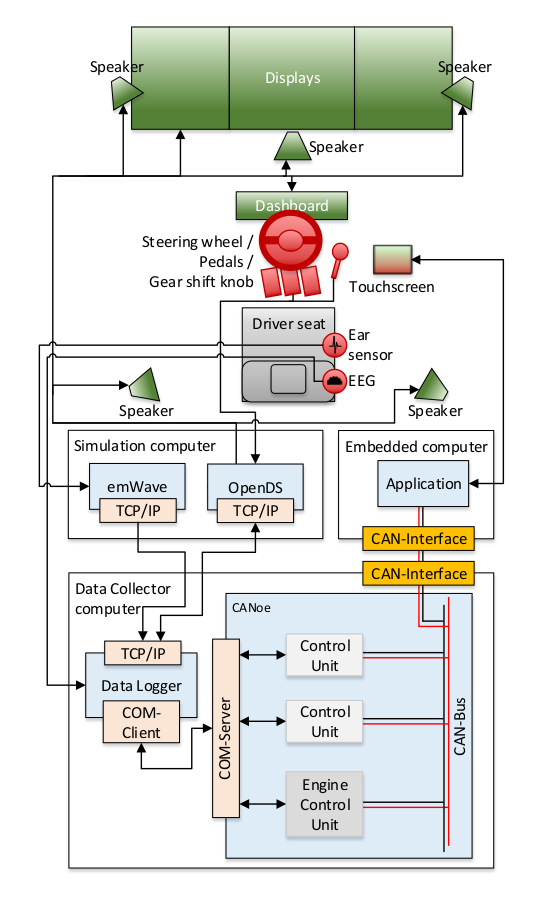
\includegraphics[width=\columnwidth]{architecture}
    \caption[Aufbau des Simulators]{Der Aufbau des Simulators der \acl{RTU} mit den drei Rechnern für die Simulation, Datensammlung und Applikation. \label{fig:architecure}}
  \end{center}
\end{figure}

Die Anwendung selbst wird in Python 2.7 \footnote{\url{https://www.python.org}} realisiert. Python ist OpenSource, lässt sich leicht lernen und der Code ist, dank des ausgefeilten Sprachkonzepts, gut lesbar. Wie schon angemerkt, ist dies für Hochschulprojekte eine wichtige Eigenschaft, da es häufig zu Personalwechseln kommt. Für Python existieren eine Vielzahl an Bibliotheken für wissenschaftliche Anwendungen. Für das Projekt werden unter anderem die SciPy\footnote{\url{http://www.scipy.org}}, welche sich an der Funktionalität von Matlab orientiert, oder die MachineLearning-Bibliothek PyBrain\footnote{\url{http://pybrain.org}} genutzt. Python läuft auf allen gängigen Betriebssystemen (Windows, Mac oder Linux) wenn der passende Python-Interpreter installiert ist. Weiterhin existieren Scripte, um eine Anwendung auch auf anderen Plattform lauffähig zu machen (Android, IPhone, etc.). Als Scriptsprache ist Python nicht ganz so schnell, als eine kompilierte Sprache, liefert jedoch ausreichende Performance. Weiterhin kann eine Python Anwendung in ByteCode kompiliert werden, um die Geschwindigkeit weiter zu steigern. 

Die komplette Anwendung ist mit docstrings (Dokumentation im Code) versehen und über eine HTML Seite abrufbar. Weiterhin sind alle wichtigen Codestellen durch Unittests abgesichert. Um den Einstieg in manche Themengebiete zu erleichtern, sind einfach Beispiele und Visualisierungen implementiert. Der Komplette Code ist unter Versionskontrolle in einem git-Repository

Die Anwendung fügt sich nahtlos in die Simulationsumgebung ein, kann aber auch Standalone betrieben werden. Das CAN-Interface kann die EEG-Rohdaten direkt via http empfangen und auf den CAN-Bus legen, als wäre das EEG ein Fahrzeugsensor. Die EEG-Daten können von der Anwendung wieder vom CAN-Bus gelesen werden und dann entsprechend weiterverarbeitet werden. Der http-Server kann auch direkt angesprochen werden. Somit sind Datenbeschaffung (EEG-Rohdaten) und Verarbeitung getrennt und können auf unterschiedlichen Geräten ausgeführt werden.

\begin{itemize}
\item SWE-Process
\item Anforderungen
\item Funktionen
\item Software Infrastruktur
\end{itemize} 